\documentclass[12pt]{report}

\usepackage[utf8]{inputenc}
\usepackage{amsmath}
%\usepackage{ae}
\usepackage{graphicx}
\usepackage{color}
\usepackage{tikz}
%\usepackage{bbm}
%\usepackage[swedish]{babel}
\newcommand{\N}{\ensuremath{\mathbbm{N}}}
\newcommand{\Z}{\ensuremath{\mathbbm{Z}}}
\newcommand{\Q}{\ensuremath{\mathbbm{Q}}}
\newcommand{\R}{\ensuremath{\mathbbm{R}}}
\newcommand{\C}{\ensuremath{\mathbbm{C}}}
\renewcommand{\d}{\ensuremath{\mathrm{d}}}
\newcommand{\e}{\ensuremath{\mathrm{e}}}
\renewcommand{\L}{\ensuremath{\mathcal{L}}}
\renewcommand{\i}{\ensuremath{i}}
\newcommand{\ket}[1]{|#1\rangle}
\newcommand{\bra}[1]{\langle#1|}
\newcommand{\braket}[2]{\bra{#1}#2\rangle}
\newcommand{\bracket}[3]{\bra{#1}#2\ket{#3}}
\newcommand{\fig}[3]{
\begin{figure}
\centering
\includegraphics{figs/#1}
\caption{#2}
\end{figure}
}


\title{Holographic Superconductivity}
\author{Petter Säterskog}
\begin{document}
\maketitle
\tableofcontents

\section{Introduction}
The AdS-CFT correspondence was conjectured in 1997 \cite{Maldacena:1997re}. It relates the physics of a string theory in Anti de Sitter space (AdS) to a conformal field theory (CFT) on the boundary of the AdS space.

Strong coupling

High TC Superconductors
\section{The Correspondence}
The correspondence can be formulated by the GKPW equation \cite{Witten:1998qj}
\begin{equation}
 Z_{\text{cft}}=Z_{\text{strings}}
\label{GKPW}
\end{equation}
where $Z_{\text{cft}}$ is the partition function of the boundary theory and $Z_{\text{strings}}$ is the partition function of the bulk theory at the same temperature. The relation between the Lagrangians of the theories are unknown but the boundary values of fields in the bulk theory corresponds to fields in the CFT.
\subsection{Partition Function}
The partition function is a concept from statistical physics. It is for a quantum-mechanical system defined as
\begin{equation}
 Z(\beta)=\mathrm{tr}(\e^{-\beta\hat{H}})
\end{equation}
where $\hat{H}$ is the time independent Hamiltonian and $\beta=(k_BT)^{-1}$ where $K_B$ is Boltzmann's constant and $T$ is the temperature. This is similar to the trace of the time-evolution operator $\hat{U}(t_2,t_1)$ evolving a state from time $t_1$ to $t_2$
\begin{equation}
 \mathrm{tr}(\hat{U}(t_2,t_1))=\mathrm{tr}(\e^{-\i\frac{(t_2-t_1)\hat{H}}{\hbar}})=f(t_2-t_1).
\end{equation}
The partition function can then be obtained as the analytical extension of $f$,
\begin{equation}
 Z(\beta)=f(-\i\beta\hbar).
\end{equation}
The trace of the time evolution operator can be calculated as an integral over configuration space which in our case will be fields configurations $\psi$,
\begin{equation}
 f(t)=\int \mathcal{D}[\psi] \bracket{\psi}{\hat{U}(t,0)}{\psi}.
\end{equation}
The time-evolution operator can be calculated using Feynman's path integrals \cite{feynman1965quantum},
\begin{equation}
 \bracket{\psi_2}{\hat{U}(t,0)}{\psi_1}=\int_{\psi_1}^{\psi_2} \mathcal{D}[\psi(t)]\e^{\frac{\i}{\hbar}S[\psi(t)]}
\end{equation}
where $S[\psi(t)]$ is the action of the path through field configurations $\psi(t)$. Combining these results tells us that the trace $f(t)$ can be calculated as a periodic time path integral with period $t$
\begin{equation}
 f(t)=\int_0^t \mathcal{D}[\psi(t)]\e^{\frac{\i}{\hbar}S[\psi(t)]}.
\end{equation}
Only paths of extremal action will contribute to this in the classical limit because of the oscillatory behaviour of the exponential. Let $\psi_\mathrm{c}(t)$ be the path that extremizes the action and expand the exponent as a Taylor series around this
\begin{equation}
\begin{split}
 S[\psi_\mathrm{c}(t)+\psi(t)]=S[\psi_\mathrm{c}(t)]+\frac{\psi(t)^2}{2!}\frac{\delta^2}{\delta\psi(t)^2} S[\psi_\mathrm{c}(t)]+
\frac{\partial_t\psi(t)^2}{2!}\frac{\delta^2}{\delta(\partial_t\psi(t))^2} S[\psi_\mathrm{c}(t)]+O(\psi(t)^3)
\end{split}
\end{equation}
The functional derivative of the action is just the ordinary derivative of the Lagrangian function. TODO
The partition function is in the classical limit
\begin{equation}
 Z(\beta)=f(-\i\beta\hbar)\underbrace{=}_{classical} \e^{\frac{i}{\hbar}S_c}
\end{equation}
where $S_c$ is the action of classical periodic path with period $-\i\beta\hbar$.
\subsection{Expectation Values}
The boundary values of the bulk fields correspond to fields in the CFT. Expectation values of observables in the CFT can be calculated using a generating functional $Z[J]$. This is a partition function for a system with a perturbed Lagrangian $\L_J(x)=\L(x)+J(x)O(x)$. Here $O(x)$ is a local operator on the fields. The generating functional can be regarded an expectation value of a system with the original Lagrangian $\L$.
\begin{equation}
\begin{split}
 Z[J]&=\int_0^{-\i\beta\hbar} \mathcal{D}[\psi(t)]\e^{\frac{\i}{\hbar}\int \L(\psi(x))+J(x)O(\psi(x))}\\
&=Z[0]\int_0^{-\i\beta\hbar} \mathcal{D}[\psi(t)]\frac{\e^{\frac{\i}{\hbar}\int \L(\psi(x))}}{Z[0]}\e^{\frac{\i}{\hbar}\int J(x)O(\psi(x))}\\
&=Z[0]\langle\e^{\frac{\i}{\hbar}\int J(x)O(\psi(x))}\rangle
\end{split}
\end{equation}
Taking a functional derivative of this gives:
\begin{equation}
\begin{split}
 \frac{\delta}{\delta J}\log(Z[J])|_{J=0}&=\frac{Z[0]\langle\frac{\i}{\hbar}O(\psi(x))\e^{\frac{\i}{\hbar}\int J(x)O(\psi(x))}\rangle}{  Z[0]\langle\e^{\frac{\i}{\hbar}\int J(x)O(\psi(x))}\rangle }\big |_{J=0}\\
&=\frac{\i}{\hbar}\langle O(\psi(x))\rangle\label{expectation}
\end{split}
\end{equation}
The partition functions of the bulk and boundary theories are the same even for a perturbed Lagrangian. Both Lagrangians are then perturbed. Expectation values of operators of the boundary theory can thus be calculated using the partition function for the bulk theory. It is though not trivial to figure out what fields in the bulk theory corresponds to what operators in the boundary theory
\section{Solution}
We wish to compute expectation values of the CFT. The field theory is a strongly coupled quantum field theory and the expectation values are thus difficult to compute directly. The expectation values can though be calculated using \eqref{expectation} and the partition function can be obtained from the GKPW equation, \eqref{GKPW}.\\

The partition function of the bulk theory must then be calculated. This is in our case easier, TODO reference, since this theory can be treated in a classical limit. But the equations of motion must still be calculated and the solutions must be translated to expectation values for the CFT. This section is devoted to the theory of how this is done.
\subsection{Metric}
The precise form of the bulk Lagrangian that corresponds to the boundary theory we are interested in is unknown. The string theory is gravitational and the Lagrangian thus has an unknown parameter that is the Newton's constant $G$. This is assumed to be small so that we are in a so called ``probe limit''. We will later see when this assumption can't be trusted, TODO. The prope limit lets us solve the equations of motion for the metric independently of the other fields. We are looking for an equilibrium solution at a finite temperature $T$ and the solution is then known to be a black hole, the Schwarzschild metric in AdS space. The metric looks like this in a particular choice of coordinates where the radial coordinate $z$ is 0 at the boundary and $z_h$ at the horizon
\begin{equation}
 \d s^2=g_{ab}\d x^a\d x^b=\frac{L^2}{z^2}\left(\frac{\d z^2}{f(z)}-f(z)\d t^2+\d \mathbf{x}^2\right).
\end{equation}
Here $f(z)=1-z^dz_h^{-d}$ and $d$ is the dimension of the boundary.
\subsection{Boundary Behaviour}
The bulk Lagrangian considered will contain different fields and depend both on the fields and their first derivatives. Consider a field $\psi$ with a mass term $-\partial_a\psi^2$ and a potential term $V(\psi)$. The classical solution is the one that extremizes the action. The action integral contains the metric as an integration measure
\begin{equation}
 S=\int\d x\sqrt{|\det g_{ab}|}\L.
\end{equation}
The Euler-Lagrange equation is obtained by varying the action. The integration measure can then be regarded as part of the Lagrangian or covariant derivatives can be used in the derivation of the Euler-Lagrange equation. The end result is in any case
\begin{equation}
\frac{2\partial_a\partial^a\psi}{z^2}-\frac{4\partial^z\psi}{z^3}-\partial_\psi V(\psi)=0.
\end{equation}
We will be interested in boundary systems with translation symmetry so $\psi$ is assumed to be a function of $z$, TODO motivate more. The equation of motion then becomes
\begin{equation}
\begin{split}
\frac{2\psi''(z)g^{zz}}{z^2}-\frac{4\psi'(z)g^{zz}}{z^3}-\partial_\psi V(\psi(z))=\\
=\frac{2\psi''(z)f(z)}{L^2}-\frac{4\psi'(z)f(z)}{zL^2}-\partial_\psi V(\psi(z))=\\
=\frac{2\psi''(z)(1-z^dz_h^{-d})}{L^2}-\frac{4\psi'(z)(1-z^dz_h^{-d})}{zL^2}-\partial_\psi V(\psi(z))
\end{split}
\end{equation}

\section{Application}
Classicallity
scalar example
show 4.68 from GKPW and classicallity assumption. Possible for general lagrangian?
\section{Application to Superconductor}
The Lagrangian used is
\begin{eqnarray}
 \mathcal{L}=&-\frac{1}{4}F_{ab}F^{ab}-m^2\psi\overline{\psi}-D_a\psi\overline{D^a\psi}
+\gamma C_{abcd}F^{ab}F^{cd}+\alpha_1(F_{ab}F^{ab})^2\nonumber\\
&+\alpha_2F^a_bF^b_cF^c_dF^d_a
\end{eqnarray}
where $D_a$ is the gauge covariant derivative $D_a=\nabla_a-iA_a$ and $F_{ab}=\partial_aA_b-\partial_bA_a$. This Lagrangian is invariant under a U(1) gauge transformation
\begin{eqnarray}
 \psi&\rightarrow&\mathrm{e}^{i\theta(x)}\psi\\
 A_a&\rightarrow& A_a+\nabla_a\theta(x).
\end{eqnarray}
This lets us make a choice of gauge, $\nabla_aA^a=0$, the Lorentz gauge. The gauge is still not completely fixed, a gauge transformation $\theta(x)$ such that $\nabla_a\nabla^a\theta(x)=0$ can still be done without violating the gauge condition.
The Lagrangian is also evidently Lorentz invariant imposing Lorentz invariance of the boundary theory.
\section{Numerical solution of bulk equations}
The bulk field equations are obtained by varying the bulk Lagrangian with respect to all the fields. This can be done with the Euler-Lagrange equation since the action does not contain any higher derivatives. The Euler-Lagrange equation for a scalar field $\phi$ states
\begin{equation}
 \partial_a\left(\frac{\partial\mathcal{L}}{\partial(\partial_a\phi)}\right)-\frac{\partial\mathcal{L}}{\partial\phi}.
\end{equation}


First consider a system with $A_r=A_x=A_y=0$. The field equations obtained by varying the fields $\psi$, $\phi$ are respectively
\begin{eqnarray}
0=&\psi \left(- \frac{m^{2}}{\operatorname{f}\left(r\right)} + \frac{\phi^{2}}{\operatorname{f}^{2}\left(r\right)}\right) + \frac{\partial^{2}}{\partial^{2} r}  \psi\nonumber\\&+\left(\frac{\frac{\partial}{\partial r} \operatorname{f}\left(r\right)}{\operatorname{f}\left(r\right)} + \frac{2}{r}\right) \frac{\partial}{\partial r} \psi
\end{eqnarray}
\begin{eqnarray}
0=&- 2 \frac{\phi \psi^{2} r^{2}}{\operatorname{f}\left(r\right)} + r^{2} \frac{\partial^{2}}{\partial^{2} r}  \phi + 2 r \frac{\partial}{\partial r} \phi.
\end{eqnarray}
\fig{O2_T}{A picture}
\section{test}


\begin{figure}
\centering
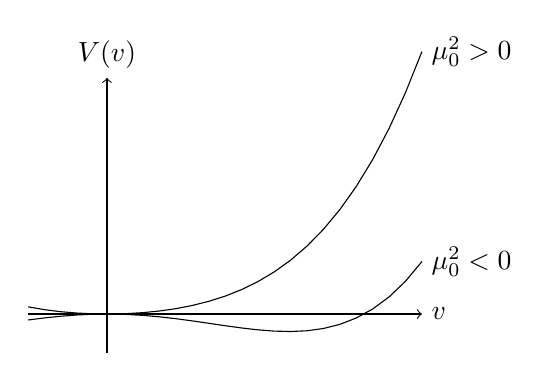
\begin{tikzpicture}
    \draw[->] (-1,0) -- (4,0) node[right] {$v$};
    \draw[->] (0,-0.5) -- (0,3) node[above] {$V(v)$};
    \draw plot[domain=-1:4] (\x,\x*\x*\x*\x/128-\x*\x/12) node[right] {$\mu_0^2<0$};
    \draw plot[domain=-1:4] (\x,\x*\x*\x*\x/128+\x*\x/12) node[right] {$\mu_0^2>0$};
\end{tikzpicture}
\caption{\label{pot}The potential used by Goldstone\cite{McGreevy:2009xe} which also is the Higgs potential. Note the minimum not being at $v=0$ giving a spontaneously broken symmetry.}
\end{figure}

\bibliographystyle{unsrt}
\bibliography{report}
\end{document}